% Copyright 2004 by Till Tantau <tantau@users.sourceforge.net>.
%
% In principle, this file can be redistributed and/or modified under
% the terms of the GNU Public License, version 2.
%
% However, this file is supposed to be a template to be modified
% for your own needs. For this reason, if you use this file as a
% template and not specifically distribute it as part of a another
% package/program, I grant the extra permission to freely copy and
% modify this file as you see fit and even to delete this copyright
% notice. 

\documentclass{beamer}

\usepackage{kotex}
\usepackage{graphicx,psfrag,amsfonts,amsmath,amssymb}
\usepackage{multicol}
%\usepackage{algorithm,algorithmic}
\usepackage{algorithm2e}

% There are many different themes available for Beamer. A comprehensive
% list with examples is given here:
% http://deic.uab.es/~iblanes/beamer_gallery/index_by_theme.html
% You can uncomment the themes below if you would like to use a different
% one:
%\usetheme{Dresden}
%\usetheme{AnnArbor}
%\usetheme{Antibes}
%\usetheme{Bergen}
%\usetheme{Berkeley}
%\usetheme{Berlin}
%\usetheme{Boadilla}
%\usetheme{boxes}
%\usetheme{CambridgeUS}
%\usetheme{Copenhagen}
%\usetheme{Darmstadt}
%\usetheme{default}
%\usetheme{Frankfurt}
%\usetheme{Goettingen}
%\usetheme{Hannover}
%\usetheme{Ilmenau}
%\usetheme{JuanLesPins}
%\usetheme{Luebeck}
%\usetheme{Madrid}
%\usetheme{Malmoe}
%\usetheme{Marburg}
%\usetheme{Montpellier}
%\usetheme{PaloAlto}
%\usetheme{Pittsburgh}
%\usetheme{Rochester}
%\usetheme{Singapore}
%\usetheme{Szeged}
%\usetheme{Warsaw}
\usetheme{metropolis}

%\usecolortheme{lily}
\usefonttheme[onlymath]{serif}	% 수식 설정!!
\setbeamertemplate{section in toc}[sections numbered]

\title{Functional Logistic Regression with Sparse Functional PCA Method}
%\date{\today}
\date[Short Occasion]{August 21, 2019}
\author{Hyunsung Kim}
\institute{Department of Statistics\\ Chung-Ang University}

% A subtitle is optional and this may be deleted
\subtitle{}

%\author{F.~Author\inst{1} \and S.~Another\inst{2}}
% - Give the names in the same order as the appear in the paper.
% - Use the \inst{?} command only if the authors have different
%   affiliation.

%\institute[Universities of Somewhere and Elsewhere] % (optional, but mostly needed)
%{
%  \inst{1}%
%  Department of Computer Science\\
%  University of Somewhere
%  \and
%  \inst{2}%
%  Department of Theoretical Philosophy\\
%  University of Elsewhere}
% - Use the \inst command only if there are several affiliations.
% - Keep it simple, no one is interested in your street address.

%\date{Conference Name, 2013}
% - Either use conference name or its abbreviation.
% - Not really informative to the audience, more for people (including
%   yourself) who are reading the slides online

\subject{Functional Data Analysis}
% This is only inserted into the PDF information catalog. Can be left
% out. 

% If you have a file called "university-logo-filename.xxx", where xxx
% is a graphic format that can be processed by latex or pdflatex,
% resp., then you can add a logo as follows:

% \pgfdeclareimage[height=0.5cm]{university-logo}{university-logo-filename}
% \logo{\pgfuseimage{university-logo}}

% Delete this, if you do not want the table of contents to pop up at
% the beginning of each subsection:
\AtBeginSubsection[]
{
  \begin{frame}<beamer>{Outline}
    \tableofcontents[currentsection,currentsubsection]
  \end{frame}
}

\def \bY {\mathbf{Y}}
\def \by {\mathbf{y}}
\def \bX {\mathbf{X}}
\def \bB {\mathbf{B}}
\def \bD {\mathbf{D}}
\def \bbeta {\boldsymbol{\beta}}
\def \btheta {\boldsymbol{\theta}}
\def \bTheta {\boldsymbol{\Theta}}
\def \bepsilon {\boldsymbol{\epsilon}}
\def \balpha {\boldsymbol{\alpha}}
\def \bgamma {\boldsymbol{\gamma}}
\def \bGamma {\boldsymbol{\Gamma}}
\def \bR {\boldsymbol{R}}
\def \bZ {\boldsymbol{Z}}
\def \bG {\boldsymbol{G}}
\def \bu {\boldsymbol{u}}
\def \bV {\boldsymbol{V}}


% Let's get started
\begin{document}

\begin{frame}
  \titlepage
\end{frame}

\begin{frame}{Outline}
  \tableofcontents
  % You might wish to add the option [pausesections]
\end{frame}

% Section and subsections will appear in the presentation overview
% and table of contents.
\section{Introduction}
\begin{frame}{Introduction}
	\begin{block}{Temporal gene expression data}
		\vspace{0.1cm}
		\begin{itemize}
			\item {
				The data was measured at $18$ equal time points($0, 7, ..., 119$).
			}
			\item {
				From this dense data, We generate 100 datasets based on the functional PCs. 
			}
		\end{itemize}
	\end{block}
	\begin{block}{Classification for the simulated data}
		\vspace{0.1cm}
		\begin{itemize}
			\item {
				We compute FPC scores using sparse functional PCA method.
			}
			\item {
				Using the above FPC scores, we perform classification using the functional logistic regression.
			}
		\end{itemize}
	\end{block}
\end{frame}


\section{Methods}
\begin{frame}{Methods}
	\begin{block}{The Sparse Functional PCA}
		\vspace{0.1cm}
		\begin{itemize}
			\item {
				It can be applied the curves measured at irregular or sparse time points.
			}
			\item {
				 James \textit{et al.} (2001) used the reduced rank model to solve the functional PC problem.
			}
			\item {
				To fit above model, \texttt{EM} algorithm was used.
			}
		\end{itemize}
	\end{block}
\end{frame}

\begin{frame}{Methods}
	\begin{block}{Functional Logistic Regression}
		\vspace{0.1cm}
		$$ Y_i = \pi_i + \epsilon_i, \hspace{0.3cm} i=1,\dots,n $$
		where $Y_i=1$, if the curve $\in G_1$ and $Y_i=0$, if the curve $\in G_2$,
		%\vspace{-0.3cm}
		$$ \begin{aligned}
		   \pi_i &= P(Y=1|X=\boldsymbol{x}_i)\\
			 	  &= \frac{ \exp[\alpha + \int_T \beta(t)x_i(t) dt] }{1 + \exp[\alpha + \int_T \beta(t)x_i(t) dt]}
		\end{aligned}  $$
		with $X:T \rightarrow \mathbb{R}$ is the predictor, $\alpha$ is an intercept parameter, $\boldsymbol\beta : T \rightarrow \mathbb{R}$ is a coefficient function, and $\epsilon_i$ is the independent errors with zero mean.
	\end{block}
\end{frame}

\begin{frame}{Methods}
	\begin{block}{Functional Logistic Regression with functional PC approach}
		\vspace{0.1cm}
		$$ Y_i = \pi_i + \epsilon_i, \ i=1,\dots,n $$
		where $Y_i=1$, if the curve $\in G_1$ and $Y_i=0$, if the curve $\in G_2$,
		%\vspace{-0.3cm}
		$$ \pi_i = \frac{ \exp[\alpha + \sum_{k=1}^K \beta_k\xi_{ik}] }{1 + \exp[\alpha + \sum_{k=1}^K \beta_k\xi_{ik}]}, \ i=1,\dots,n $$
		with $\alpha$ is an intercept parameter and $\boldsymbol\beta$ is a coefficient function, $\xi_{ik}$ is $k$th FPC score for the $i$th individual, and $\epsilon_i$ is the independent errors with zero mean.
	\end{block}
\end{frame}



\section{Simulation}
\begin{frame}{Simulation}
	\begin{block}{The simulated datasets}
		\vspace{0.1cm}
		\begin{itemize}
			\item {
				The $100$ datasets are simulated from the first $5$ estimated FPCs from the temporal gene expression data.
			}
			\item {
				 Each dataset has $200$ curves with 2 groups($G_1, G_2$)
				 and is randomely divided to $100$ training and test sets for each.
			}
			\item {
				We perform the functional logistic regression for the training sets, and predict for the test sets.
			}
		\end{itemize}
	\end{block}
\end{frame}

\begin{frame}{Simulation}
	\begin{figure}[h] %%% t: top, b: bottom, h: here
		\begin{center}
			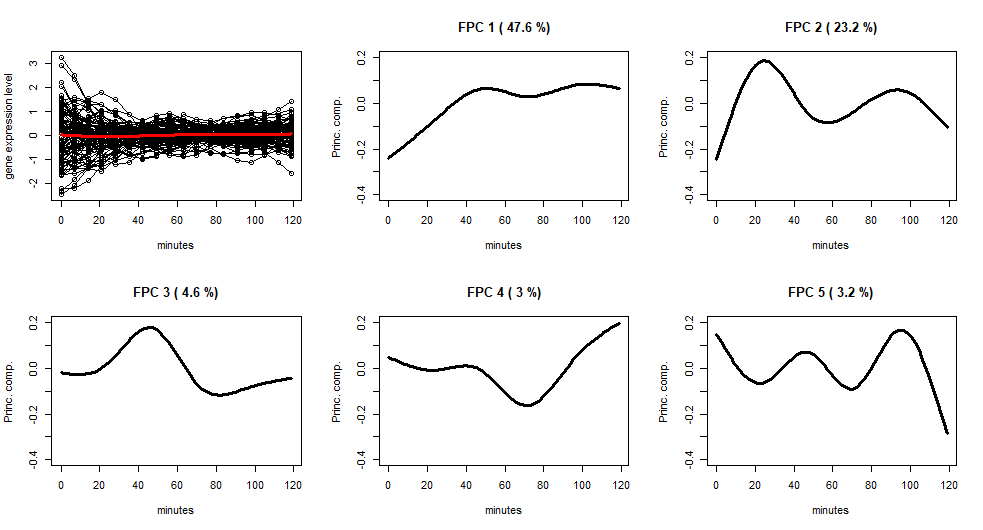
\includegraphics[width=1\linewidth]{img/1.png}
		\end{center}
		\label{fig:long}
		\label{fig:onecol}
		\caption{The mean curve and 5 FPC functions for $1$st training set}
	\end{figure}
\end{frame}

\begin{frame}{Simulation}
	\begin{figure}[h] %%% t: top, b: bottom, h: here
		\begin{center}
			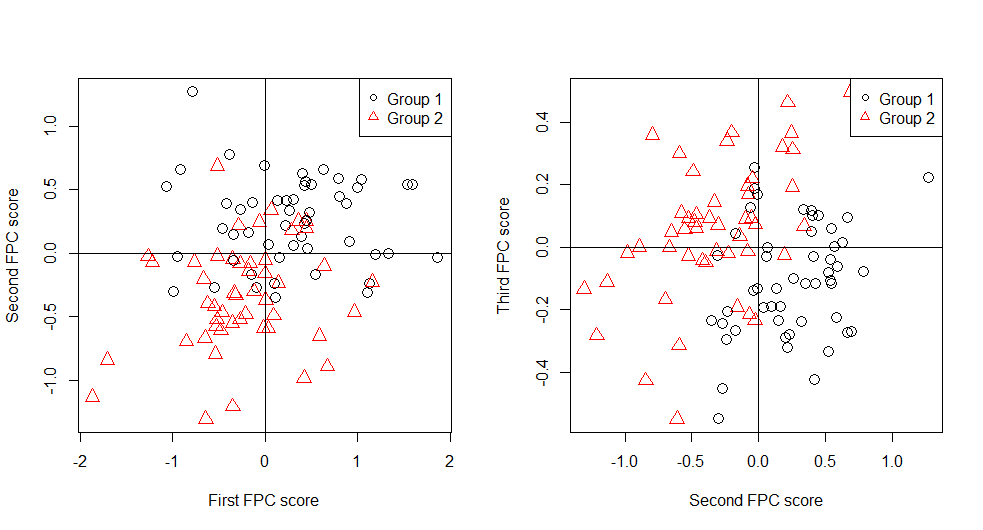
\includegraphics[width=1\linewidth]{img/3.png}
		\end{center}
		\label{fig:long}
		\label{fig:onecol}
		\caption{Scatterplot of pairwise FPC scores for $1$st training dataset}
	\end{figure}
\end{frame}

\begin{frame}{Simulation}
	\begin{figure}[h] %%% t: top, b: bottom, h: here
		\begin{center}
			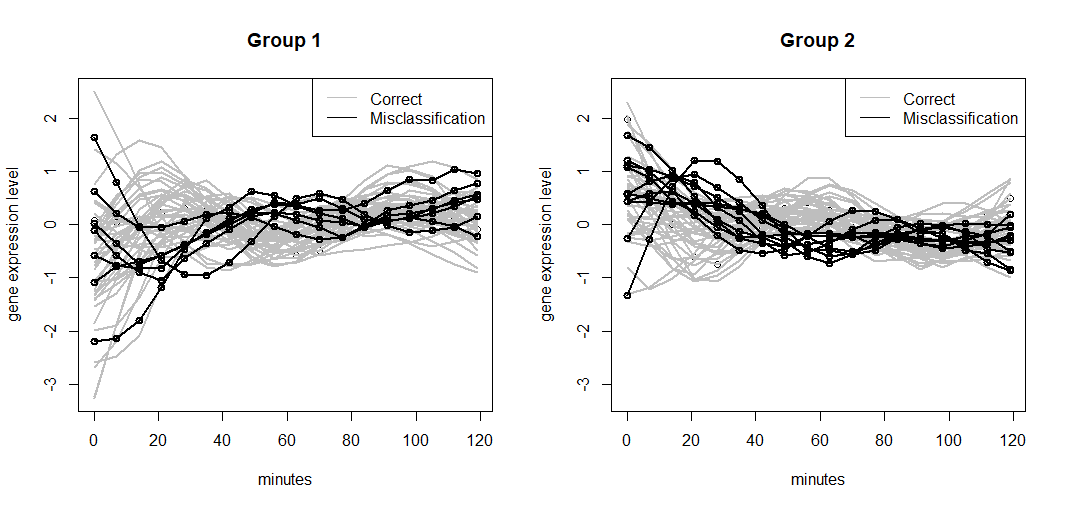
\includegraphics[width=1\linewidth]{img/2.png}
		\end{center}
		\label{fig:long}
		\label{fig:onecol}
		\caption{The curves classified by functional logistic regression for $1$st simulated dataset}
	\end{figure}
\end{frame}

\begin{frame}{Simulation}
	\begin{table}[ht]
		\caption{Classification error rates between Dense and Sparse method}
		\centering
		\tiny
		\begin{tabular}{lllllll}
			\hline
			No. of & \multicolumn{2}{l}{Group 1} & \multicolumn{2}{l}{Group 2} & \multicolumn{2}{l}{Overall} \\
			FPCs   & Dense & Sparse & Dense & Sparse & Dense & Sparse \\
			\hline
			$1$ & 32.72 (8.41) & 31.67 (0.08) & 32.70 (8.31) & 33.65 (0.08) & 32.71 (5.26) & 32.68 (0.06) \\
			$2$ & 22.16 (6.65) & 22.20 (0.08) & 22.06 (6.15) & 22.00 (0.07) & 22.11 (4.33) & 22.10 (0.05) \\
			$3$ &  7.58 (4.58) & 12.45 (0.11) &  8.26 (5.34) & 12.47 (0.09) &  7.92 (3.35) & 12.46 (0.09) \\
			$4$ &  7.14 (4.14) & 11.81 (0.09) &  7.62 (5.10) & 11.37 (0.08) &  7.38 (3.11) & 11.59 (0.08) \\
			$5$ &  7.40 (4.07) & 12.22 (0.11) &  7.86 (5.26) & 11.45 (0.08) &  7.63 (3.06) & 11.83 (0.09) \\
			\hline
		\end{tabular}
	\end{table}
\end{frame}

\begin{frame}{Simulation}
	\begin{block}{Comparison between Dense and Sparse FPCA method}
		\vspace{0.1cm}
		\begin{itemize}
			\item {
				The sparse method shows higher misclassification rate than the dense one.
			}
			\item {
				The Monte Carlo standard errors are much lower on the sparse method.
			}
			\item {
				For the data measured at all time points, the dense functional PCA method perform well than the sparse method.
			}
		\end{itemize}
	\end{block}
\end{frame}



\appendix
\section{Reference}
\begin{frame}
  \frametitle<presentation>{Reference}
    
  \begin{thebibliography}{10}
  	\beamertemplatearticlebibitems
	% Followed by interesting articles. Keep the list short. 
	 \bibitem{Someone2000}
		%GARETH M. JAMES, TREVOR J. HASTIE, CATHERINE A. SUGAR
		James G.M., Hastie T.J., Sugar C.A.
		\newblock Principal component models for sparse functional data
		\newblock {\em Biometrika}, 87(3):587--602,
		2000.
		
   	\beamertemplatearticlebibitems
		\bibitem{Someone2008}
		 Zhou L. \textit{et al.}
		 \newblock Joint modeling of paired sparse functional data using principal components
		 \newblock {\em Biometrika}, 95(3):601--619,
		 2008.
    
    \beamertemplatearticlebibitems
    \bibitem{Someone2006}
    Leng. X. and Müller. HG.
    \newblock Classification using functional data analysis for temporal gene expression data
    \newblock {\em Bioinformatics}, 22(1):68--76,
    2006.

  \end{thebibliography}
\end{frame}


% All of the following is optional and typically not needed. 
%\appendix
%\section<presentation>*{\appendixname}
%\subsection<presentation>*{For Further Reading}
%
%\begin{frame}[allowframebreaks]
%  \frametitle<presentation>{For Further Reading}
%    
%  \begin{thebibliography}{10}
%    
%  \beamertemplatebookbibitems
%  % Start with overview books.
%
%  \bibitem{Author1990}
%    A.~Author.
%    \newblock {\em Handbook of Everything}.
%    \newblock Some Press, 1990.
% 
%    
%  \beamertemplatearticlebibitems
%  % Followed by interesting articles. Keep the list short. 
%
%  \bibitem{Someone2000}
%    S.~Someone.
%    \newblock On this and that.
%    \newblock {\em Journal of This and That}, 2(1):50--100,
%    2000.
%  \end{thebibliography}
%\end{frame}

\end{document}


